
\section{Prueba de Concepto}
Para la realización de este proyecto se ha decidido crear un entorno virtual dentro de la infraestructura real donde está localizado el servicio, para poder desplegar el software Cloud Foundation y probarlo sin afectar a la configuración ni al funcionamiento general del servicio. La parte física de este entorno está formada por cuatro máquinas virtuales, que equivalen a cuatro nodos físicos con el hipervisor ESXi instalado en cada uno. También cuenta con una máquina virtual con vCenter Server para permitir el acceso al entorno, y otra máquina virtual con Windows Server 2016 donde se habilitan servicios de red como DNS,NTP o DHCP.
*****ESTRUCTURA DEL ENTORNO.
\subsection{Especificaciones del entorno}
Estas son las características de hardware y software del nuevo entorno de pruebas.
\begin{itemize}
    \item \textbf{Cuatro nodos ESXi}, cada uno con la siguiente configuración:
    \begin{itemize}
        \item Hipervisor: VMware ESXi, version 6.7.0, build 10302608
        \item Procesador: Intel(R) Xeon(R) CPU E5-2650 v4 @ 2.20GHz
        \item Memoria: 24GB
        \item Discos de almacenamiento: un disco duro arranque con 8GB de capacidad, un disco duro de 100GB y tres discos duros de 200GB.
    \end{itemize}
            \begin{figure}[h!]
            \centering
            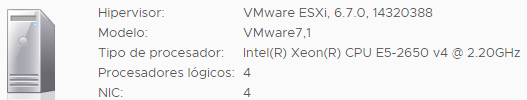
\includegraphics[width=0.85\textwidth]{imaxes/probaConcepto/caracteristicas_NODO.png}
            \caption{Características comunos a cada host.} 
            \label{fig:caracteristicasNODO}
        \end{figure}
        \FloatBarrier
    \item \textbf{Almacenamiento}: El almacenamiento está basado en el prodcuto VMware vSAN siguiendo el modelo All-Flash. Este servicio unifica los discos duros de cada host en un único almacén de datos dividido en cuatro grupos de discos donde el disco de 100 GB representa el disco de memoria caché y los tres discos de 200 GB representan los discos de capacidad. La capacidad total útil del clúster es de 2,34 TB.
    \item \textbf{Software}: Para crear la capa de virtualización, este entorno tiene instalado vSphere que contiene los componentes ya descritos [Sec.\ref{subsec:softwareinstalado}], y vSAN para la gestión del almacenamiento [Sec. \ref{subsubsect:cfcomponents}].
\end{itemize}

\subsection{Configuración Inicial}
En este apartado se expone cual es la configuración de los nodos físicos sobre red y servicios habilitados antes de realizar el despliegue de Cloud Foundation. Nodos existentes:
%%%%%%Centrar esta lista.%%%%%%%%%%%
    \begin{itemize}
        \item \textbf{Nodo 1}: sa-esxi-01.vclass.local
        \item \textbf{Nodo 2}: sa-esxi-02.vclass.local
        \item \textbf{Nodo 3}: sa-esxi-03.vclass.local
        \item \textbf{Nodo 4}: sa-esxi-04.vclass.local
    \end{itemize}
%%%%%%%%%%%%%%%%%%%%%%%%%%%%%%%%%%%

\subsubsection{Red}
\label{sec:redPrueba}
Los cuatro nodos del entorno están conectados entre si a través de tres redes, cada una con un propósito diferente. Para la distribución de los datos de cada red, se utiliza un switch virtual llamado vSwitch que da conectividad entre las máquinas virtuales y hosts del entorno (un vSwitch por red). Cada nodo tiene cuatro puertos físicos, que en este caso son virtuales ya que los nodos no son reales, los cuales se asignan a los diferentes vSwitches que se van creando para configurar la red, permitiendo asignar más de un puerto a un vSwitch para crear redundancia. Así, cada vSwitch redirigirá el tráfico por su puerto asignado. Dentro de la nomenclatura de VmWare, estos puertos se llaman \setword{\textbf{vmnicX}}{Word:vmnic} donde X es su numeración.\\
Configuración de los switches en cada nodo, esta configuración se repite en cada nodo:
\begin{itemize}
    \item \underline{vSwitch0}:
    \label{itm:managementNet}
        Red \emph{SDDC-DPortGroup-Mgmt} con IP 172.20.10.0/24.
        El nodo 1 tiene la IP 172.20.10.51, el nodo 2 la IP 172.20.10.52, el nodo 3 la IP 172.20.10.53, y el nodo 4 la IP 172.20.10.54.
        Esta red es utilizada por servicios de gestión, como el acceso SSH a los nodos, la sincronización de tiempo por NTP, acceso al servidor DNS, o el acceso a la interfaz de configuración del entorno con vSphere WebClient. Se usa a través de puertos \emph{vmkernel}.

        \begin{figure}[h!]
            \centering
            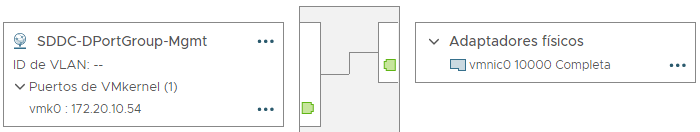
\includegraphics[width=0.85\textwidth]{imaxes/probaConcepto/vswitch0.png}
            \caption{\emph{vSwitch0} del nodo \emph{sa-esxi-01.vclass.local}} 
            \label{fig:componentesVSphere}
        \end{figure}
        \FloatBarrier
    \item \underline{vSwitch1}:
    \label{itm:vsanNet}
        Red \emph{SDDC-DPortGroup-VSAN} con IP 172.20.12.0/24.
        El nodo 1 tiene la IP 172.20.12.51, el nodo 2 la IP 172.20.12.52, el nodo 3 la IP 172.20.12.53, y el nodo 4 la IP 172.20.12.54.
        Esta red sirve para comunicar los nodos con el datastore de vSAN. Se usa a través de puertos \emph{vmkernel}.
        \begin{figure}[h!]
            \centering
            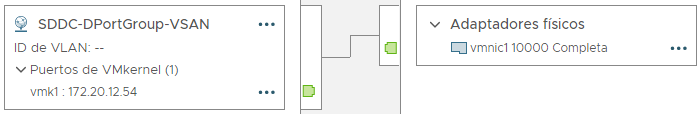
\includegraphics[width=0.85\textwidth]{imaxes/probaConcepto/vswitch1.png}
            \caption{\emph{vSwitch1} del nodo \emph{sa-esxi-04.vclass.local}} 
            \label{fig:componentesVSphere}
        \end{figure}
        \FloatBarrier
    \item \underline{vSwitch2}:
    \label{itm:machinesNet}
        Red \emph{VM Network}. No tiene ninguna IP asignada. Esta red da conectividad a las máquinas virtuales de cada nodo. Se usa a través de puertos \emph{vmportgorups}.
        \begin{figure}[h!]
            \centering
            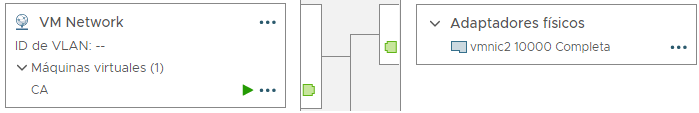
\includegraphics[width=0.85\textwidth]{imaxes/probaConcepto/vswitch2.png}
            \caption{\emph{vSwitch2} del nodo \emph{sa-esxi-04.vclass.local}} 
            \label{fig:componentesVSphere}
        \end{figure}
        \FloatBarrier
\end{itemize}

******ESQUEMA DE LOS PUERTOS**************

 Según el tipo de red que se esté añadiendo en cada vSwitch, se creará en este un tipo distinto de puerto que se conectará con el puerto físico mencionado anteriormente. Estos puertos pueden ser \setword{\emph{vmwkernel}}{Word:vmkernel} (vmkX) para el tráfico de los servicios que usan los nodos ESXi, y \textit{vmportgroup} para tráfico general de las máquinas virtuales.
 Para que un nodo tenga conectividad con otro nodo, estos deben tener configurada la misma red en sus vSwitches. 
 Inicialmente, todas las redes tienen deshabilitado el etiquetado de VLAN.\\
 Estos vSwitches descritos forman la red lógica del entorno pero por donde realmente viaja todo el tráfico es sobre la red física de la infraestructura, que está formada por un switch cuyo MTU es igual a 1500.
 
 
 \subsubsection{Servicios internos}
 
 Inicialmente, en cada host los siguientes servicios están configurados y en ejecución:
 \begin{itemize}
     \item \textbf{Direct Console UI}: permite interactuar con el host de forma local mediante una interfaz basada en texto.
     \item \textbf{ESXi Shell}: permite interactuar con los hosts de forma completa, ya sea en local o en remoto, mediante comandos. Se puede acceder a través de SSH.
     \item \textbf{SSH}: servicio que habilita el acceso a ESXi Shell de forma remota.
     \item \textbf{Load-Based Teaming}: establece una política para balancear el tráfico que pasa por cada puerto \emph{vmnic}.
     \item \textbf{NTP}: servicio que obtiene la hora actual de un servidor NTP, así todos los nodos mantienen su hora sincronizada. La sincronización se realiza con un servidor NTP con la IP 172.20.10.10.
     \item \textbf{Syslog Server}: recoge mensajes de VMkernel y otros componentes.
     \item \textbf{VMware vCenter Agent}: permite al vCenter tener acceso a cada nodo.
     \item \textbf{DNS}: servicio que está situado en un servidor con la IP 172.20.10.10. Contiene todas las redes exitentes y los nombres de cada host para que todos los componentes sean accesibles a través de la red.
 \end{itemize}
 En el entorno existe un dominio de \emph{Single Sing-On}[\ref{itm:singlesingonEX}] habilitado con el nombre \emph{vsphere.local}.\\
 
 \subsubsection{Servicios externos}
 El servidor donde se encuentran los servicios DNS, DHCP y NTP, tiene tres adaptadores de red a donde llegan cada una de las redes descritas anteriormente.\\
 El \underline{servicio DNS} cuenta con los siguientes nombres registrados:
         \begin{figure}[h!]
            \centering
            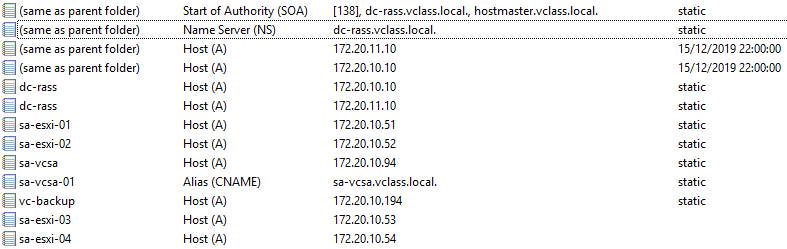
\includegraphics[width=0.95\textwidth]{imaxes/probaConcepto/nombresDNSINIcioFW.png}
            \caption{Contenido inicial \textit{forward} del DNS.} 
            \label{fig:contenidoinicialForwardDNS}
        \end{figure}
        
        \begin{figure}[h!]
            \centering
            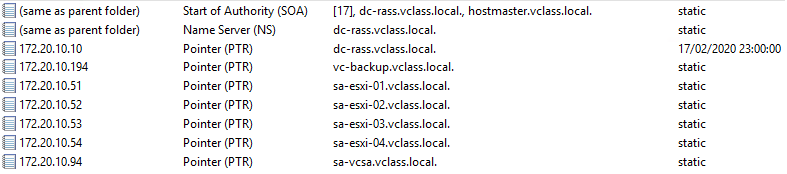
\includegraphics[width=0.95\textwidth]{imaxes/probaConcepto/dnsINICIOReverse.png}
            \caption{Contenido inicial \textit{reverse} del DNS.} 
            \label{fig:contenidoinicialReverseDNS}
        \end{figure}
        \FloatBarrier
El \underline{servicio DHCP} cuenta con la siguiente configuración:
        \begin{figure}[h!]
            \centering
            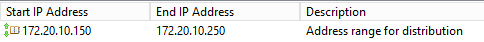
\includegraphics[width=0.85\textwidth]{imaxes/probaConcepto/scope1722010Inicio.png}
            \caption{Rango de IPs inicial para la red de 172.20.10.0/24 (Descrip. \ref{itm:managementNet}).} 
            \label{fig:dhcpInicioManage}
        \end{figure}
        \begin{figure}[h!]
            \centering
            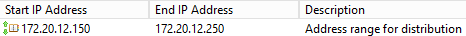
\includegraphics[width=0.85\textwidth]{imaxes/probaConcepto/scope1722012Inicio.png}
            \caption{Rango de IPs inicial para la red de 172.20.12.0/24 (Descrip. \ref{itm:vsanNet}).} 
            \label{fig:dhcpInicioSAN}
        \end{figure}
        \begin{figure}[h!]
            \centering
            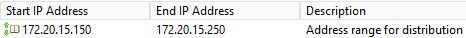
\includegraphics[width=0.85\textwidth]{imaxes/probaConcepto/scope1722015Inicio.png}
            \caption{Rango de IPs inicial para la red de 172.20.15.0/24 (Descrip. \ref{itm:machinesNet}).} 
            \label{fig:dhcpInicioMachines}
        \end{figure}
    \iffalse
        \begin{figure}[h!]
            \centering
            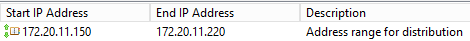
\includegraphics[width=0.85\textwidth]{imaxes/probaConcepto/scope1722011Inicio.png}
            \caption{Rango de IPs inicial para la red de 172.20.11.0/24 (Descrip. \ref{itm:machinesNet}).} 
            \label{fig:dhcpInicioMachines}
        \end{figure}
    \fi
    Para dar acceso a estos tres servicios desde cualquier componente del entorno el servidor donde se encuentran alojados debe tener al menos un adaptador de red (NIC) por cada red existente. Además, este servidor es la puerta de enlace de todos los componentes por lo que también se debe modificar su tabla de enrutamiento y para que todos los componentes del entorno se puedan comunicar entre si.\\
    *******METER FOTO DE LOS ADAPTADORES DE RED**********\\
    *******METER FOTO DE LA TABLA DE ENRUTAMIENTO.*********
    
\FloatBarrier